%!TEX root = ../Demo.tex
\chapter{预备知识}
在进行本文的叙述之前,需要预先了解一些相关的知识和定义,以便于使用更加简洁的描述方式。

一般来说,我们使用状态转移图来表示一个自动机,如图\ref{fig:state_graph}

\begin{figure}[!htbp]
    \centering
    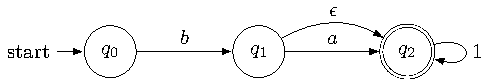
\includegraphics[width=0.7\textwidth]{state_graph}
    \caption{自动机状态转移图}
    \label{fig:state_graph}
\end{figure}

图\ref{fig:state_graph}中,自动机由$q_0$进入,接收字符“b”进入状态$q_1$,状态$q_1$接收字符“a”进入状态$q_2$,图中的两个同心圆圈住状态$q_2$表示结束状态或者接受状态,意味自动机处理字符串到达此状态时,自动机就接受当前处理的字符串,状态$q_2$上有一个指向自己的箭头,意为接收字符“1”之后,仍然指向自己。而状态$q_1$经过$\epsilon$转移到状态$q_2$,意为状态$q_1$可以不接收任何字符即可转移到状态$q_2$。图\ref{fig:state_graph}中的自动机接受的字符串为$ba(1)^*\cup b(1)^*$。

\begin{definition}
    \textbf{有限自动机}\cite{watson1993taxonomyb}:也称有限状态自动机(Finite automata,FA),有限自动机是一个6元组$(Q,V,T,E,S,F)$,其中
    \begin{itemize}
        \item $Q$ 是有限状态集;
        \item $V$ 是一个字母表;
        \item $ T \in \mathcal{P}(P\times V \times Q) $是一个转移关系;
        \item $ E \in \mathcal{P}(Q\times Q)$ 是一个$\epsilon$-转移关系(空转移,不需要接收字符即可转移);
        \item $ S \subseteq Q $是开始状态集;
        \item $ F \subseteq Q $是结束状态集;
    \end{itemize}
    字母表和函数$\mathcal{P}$的定义分别在“定义\ref{def:Alphabat}” 和 “惯例\ref{pro:mathP}”。
\end{definition}

\begin{example}
    我们可以用$M=(\{q_0,q_1,q_2\},\{b,a,1,\epsilon\},T,E,\{q_0\},\{q_2\})$来指代图\ref{fig:state_graph}中的自动机。其中,$T=\{(q_0 \times b \times q_1),(q_1\times a \times q_2),(q_2\times 1 \times q_2)\}$,$E=(q_1 \times q_2)$。
\end{example}

为了在某些情况下方便的展示状态之间的关系,也把状态转移图写成表格\cite{book1},如图\ref{fig:state_graph}中的自动机,写成表格\ref{tab:sample}:
\begin{table}[!htbp]
    \caption{状态转移函数}
    \label{tab:sample}
    \centering
    \small% fontsize
    \setlength{\tabcolsep}{4pt}% column separation
    \renewcommand{\arraystretch}{1.2}%row space 
    \begin{tabular}{l p{4em}<{\centering} p{3em}<{\centering} p{3em}<{\centering} p{3em}<{\centering} p{3em}<{\centering}} 
        \toprule%\hline 
        \multirow{2}{*}{状态说明} & \multirow{2}{*}{状态} & \multicolumn{4}{c}{输入字符} \\
		\cline{3-6}      &    &$a$ & $b$ & $1$ & $\epsilon$ \\
        %                        &        & \multicolumn{4}{c}{输入字符} \\
        %\cline{3-6}  {状态说明}  & {状态} &$a$ & $b$ & $1$ & $\epsilon$ \\
        \midrule%\hline
        开始状态(start)  & $q_0$ & -     & $q_1$  &      - &     -    \\
                        & $q_1$ & $q_2$ &    -   &    -   &    $q_2$ \\
        结束状态(accept) & $q_2$ &   -   & -      & $q_2$  &    -     \\
        \bottomrule%\hline 
    \end{tabular}
\end{table}

%\newpage
下文中将表格\ref{tab:sample}简称为转移函数。表格\ref{tab:sample}的状态之间的关系与$T=\{(q_0 \times b \times q_1),(q_1\times a \times q_2),(q_2\times 1 \times q_2)\}$,$E=(q_1 \times q_2)$一一对应。

\begin{definition}
    \textbf{确定性有限自动机}:当且仅当 
    \begin{itemize}
        \item [·] 无多重初始状态;
        \item [·] 无$\epsilon$转移;
        \item [·] 转移函数$T \in Q \times V \longrightarrow \mathcal{P} (Q) $ 不将 $Q \times V$ 映射至多重状态。
    \end{itemize}
    时有限自动机$M$是确定性的。
    公式形式表达为:
    \begin{equation}
    Det(M) \equiv ( |S| \leq 1 \land \epsilon\mbox{-} free(E) \land ( \forall q,a:q \in Q \land a \in V : |T(q,a)| \leq 1 )) 
    \end{equation}
    下文中将确定性有限自动机简称为$DFA$(Deterministic Finite Automata)。
\end{definition}

